\chapter{Contenido y Uso de Gnome Shell}
\begin{center}
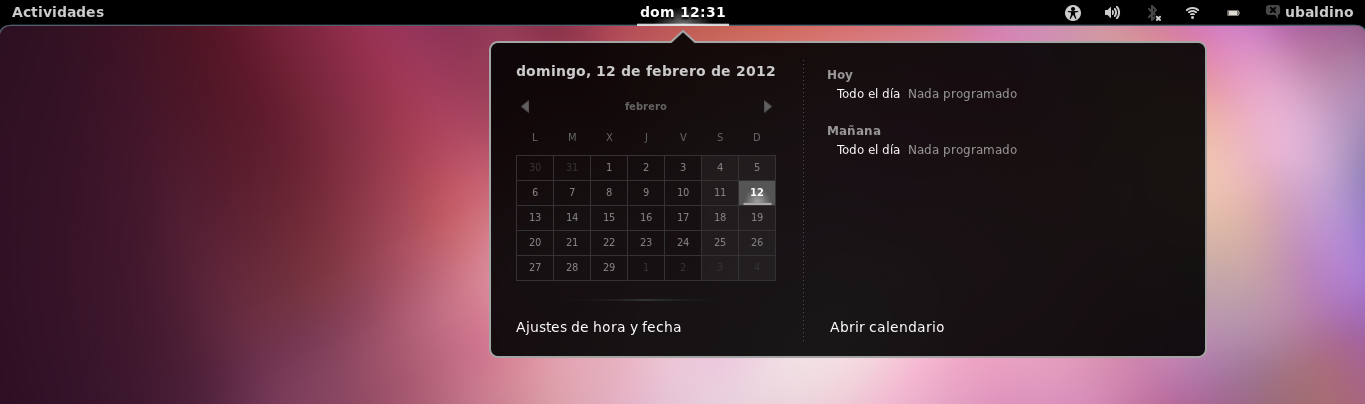
\includegraphics[scale=0.448]{img/barra.png}
\end{center}
Gnome es uno de los tantos escritorios que existen para las distribuciones basadas en linux.
En este caso UBUNTU 11.10 utiliza el escritorio o interfaz gráfica Gnome 3, y como es de esperar de un escritorio, los componentes principales del escritorio Gnome son:
\begin{itemize}
\item[-] Iconos que enlazan a archivos, carpetas o programas (accesos directos).
\item[-] Gnome Shell que es la barra de tareas y lanzador de aplicaciones. y tiene un gestor de ventanas con soporte OpenGL.
\begin{description}
\item[Gnome Shell] tiene un panel único en la parte superior, que contiene:
\begin{itemize}
 \item menú de usuario. 
 \item un botón “actividades”. 
 \item aplicaciones en ejecución.
 \item reloj.
 \item área de accesibilidad.
 \item control de volumen.
 \item información de la red.
 \item estado de la batería en el caso de un portátil.
\end{itemize}
En el arranque del sistema aparece dicho panel y el fondo de escritorio.
\end{description}
\begin{center}
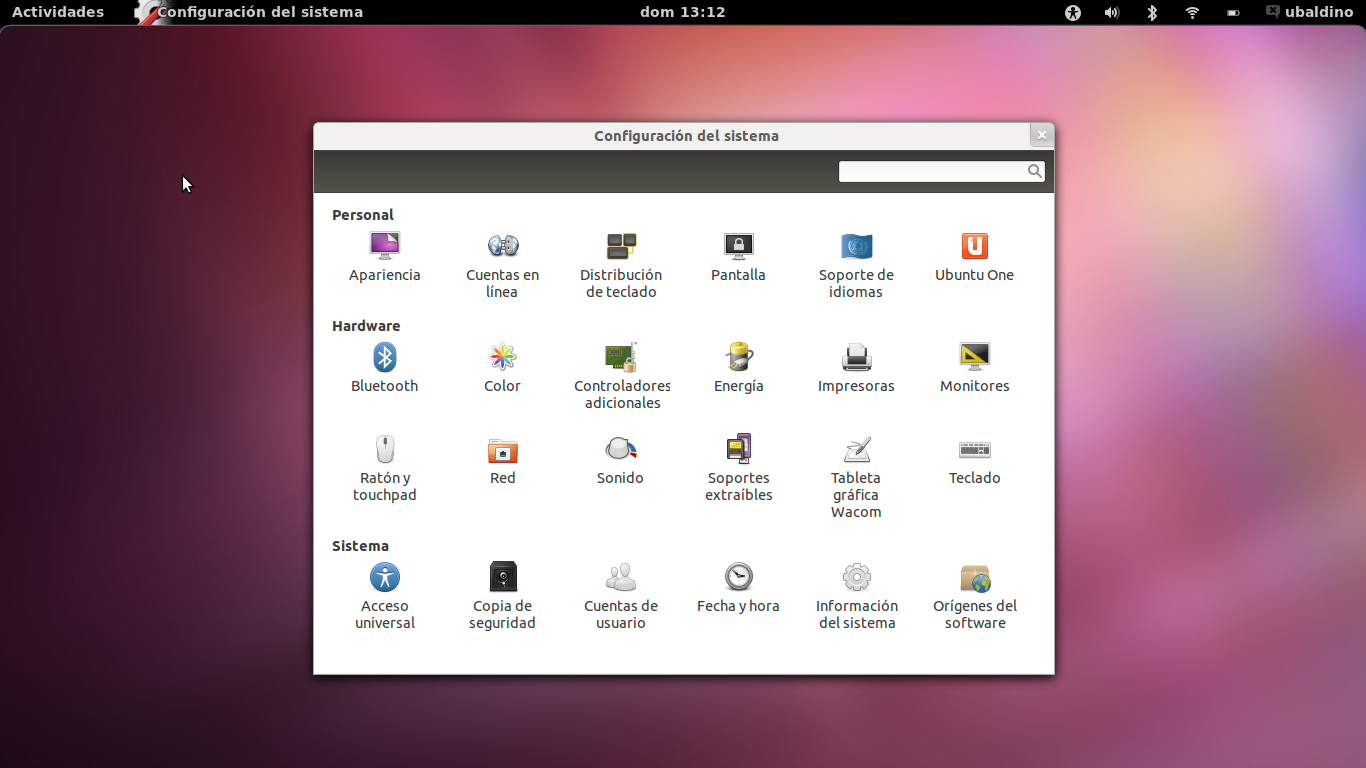
\includegraphics[scale=0.3]{img/Pantallazo3.png}
\end{center}
Al pulsar sobre “actividades” o acercar el ratón con rapidez a la esquina superior izquierda, se despliegan varios elementos nuevos:
\begin{itemize}
\item A la izquierda, un panel lanzador de aplicaciones,
\item Bajo el panel superior, un menú de dos opciones, “ventanas” y “aplicaciones”.
\item A la derecha, otro panel con una vista previa de las ventanas activas que actúa como selector de escritorios y por encima de éste, una caja de búsqueda.
\end{itemize}
Si tienes ya algún programa en ejecución, que por defecto se lanza a pantalla completa, la ventana o ventanas activas que su reducen su tamaño mostrando una leyenda informativa en la parte inferior de cada ventana. Cada acción que comporte cambios de tamaño o posición, vendrá acompañada de una elegante animación y otros efectos visuales.\\
El botón gráfico windows (ventanas), restaura la vista previa de aquellas que estén activas si las has perdido de vista por ejecutar cualquier otra acción.
\begin{center}
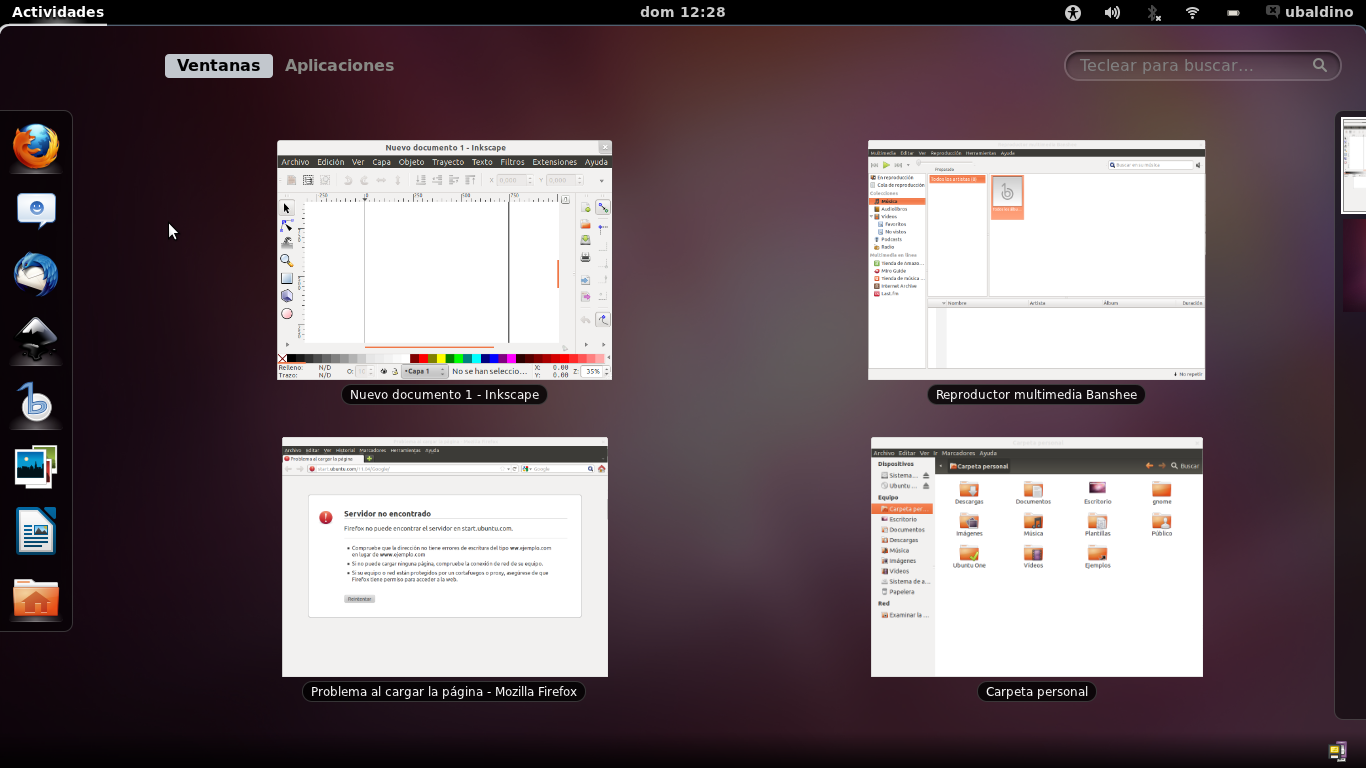
\includegraphics[scale=0.3]{img/Pantallazo4.png} 
\end{center}
El botón aplications (aplicaciones), da paso a la representación mediante iconos de los programas instalados en la máquina.
\begin{center}
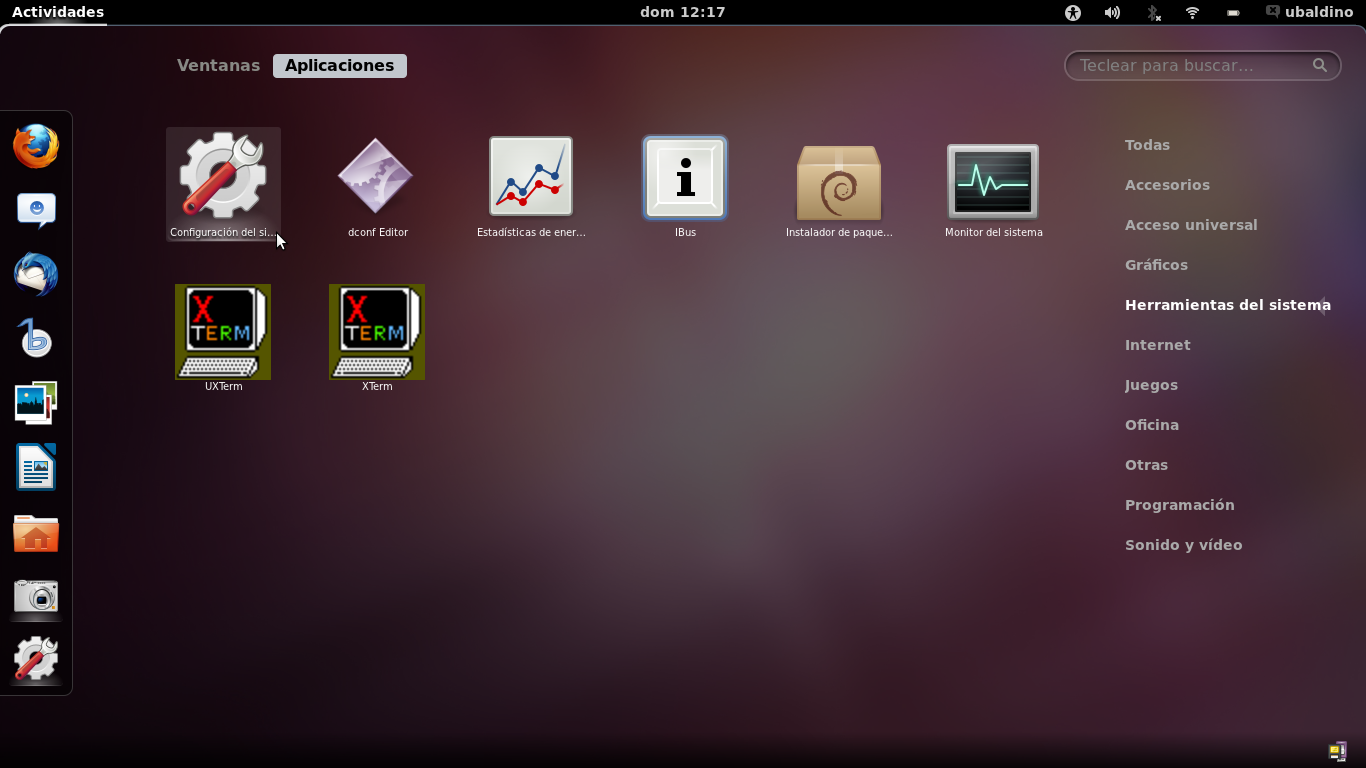
\includegraphics[scale=0.3]{img/Pantallazo5.png}
\end{center}
\underline{\bf Nota:} Note que cuando estamos en la presentación de los programas instalados en la maquina. El panel de la derecha porta un sistema de filtrado, clasificando los programas según las funcionalidades.\\

La caja de búsqueda es lo novedoso de gnome 3. Escribiendo las primeras letras de una aplicación, aparecerá de forma inmediata el icono correspondiente al programa y puedes lanzar la aplicación desde ahí. Y en la parte inferior de la pantalla muestra dos botones gráficos, que permiten extender la búsqueda en Wikipedia y Google. 
\begin{center}
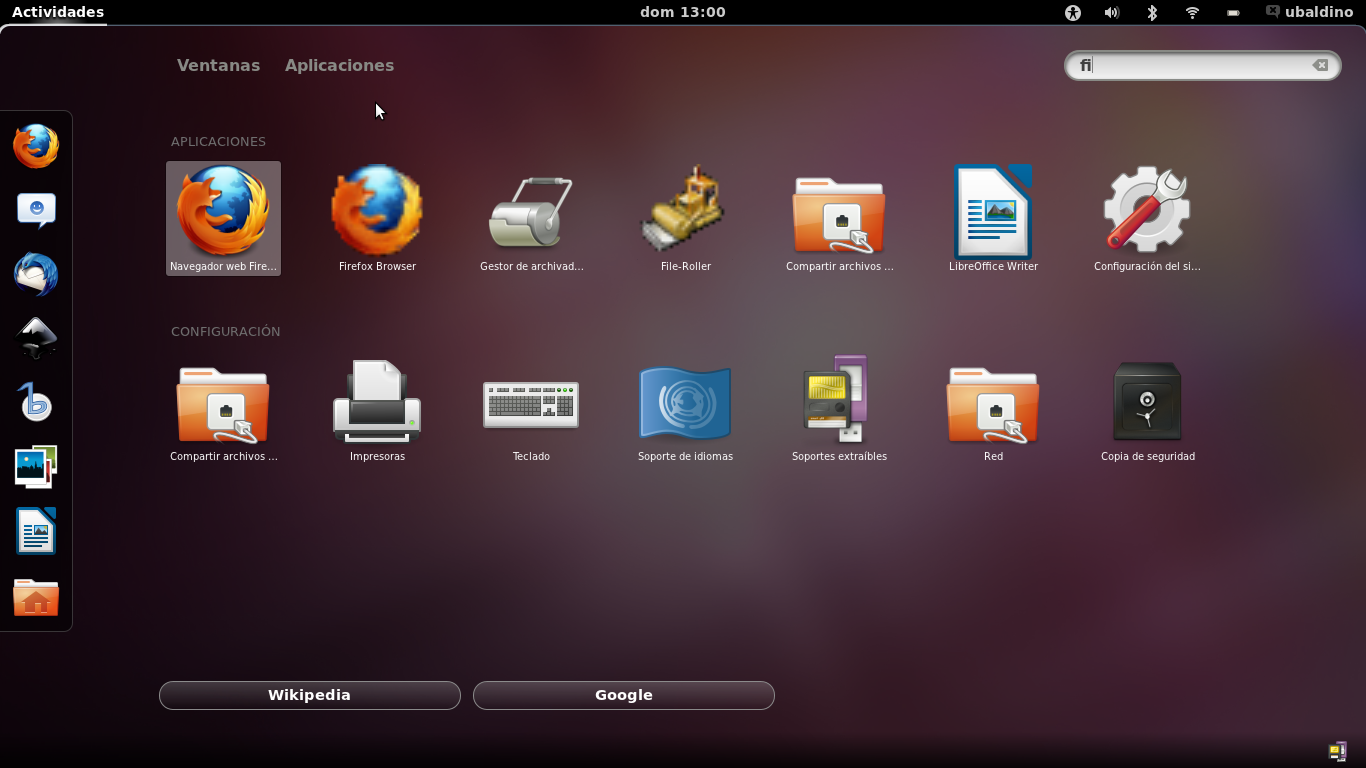
\includegraphics[scale=0.3]{img/Pantallazo6.png}
\end{center}
Por último, terminando nuestro recorrido en Gnome Shell, en la parte inferior derecha de la pantalla veremos el área de notificaciones y bandeja de mensajes, desde donde puedes contestar con el programa de mensajería instantánea.
\begin{center}
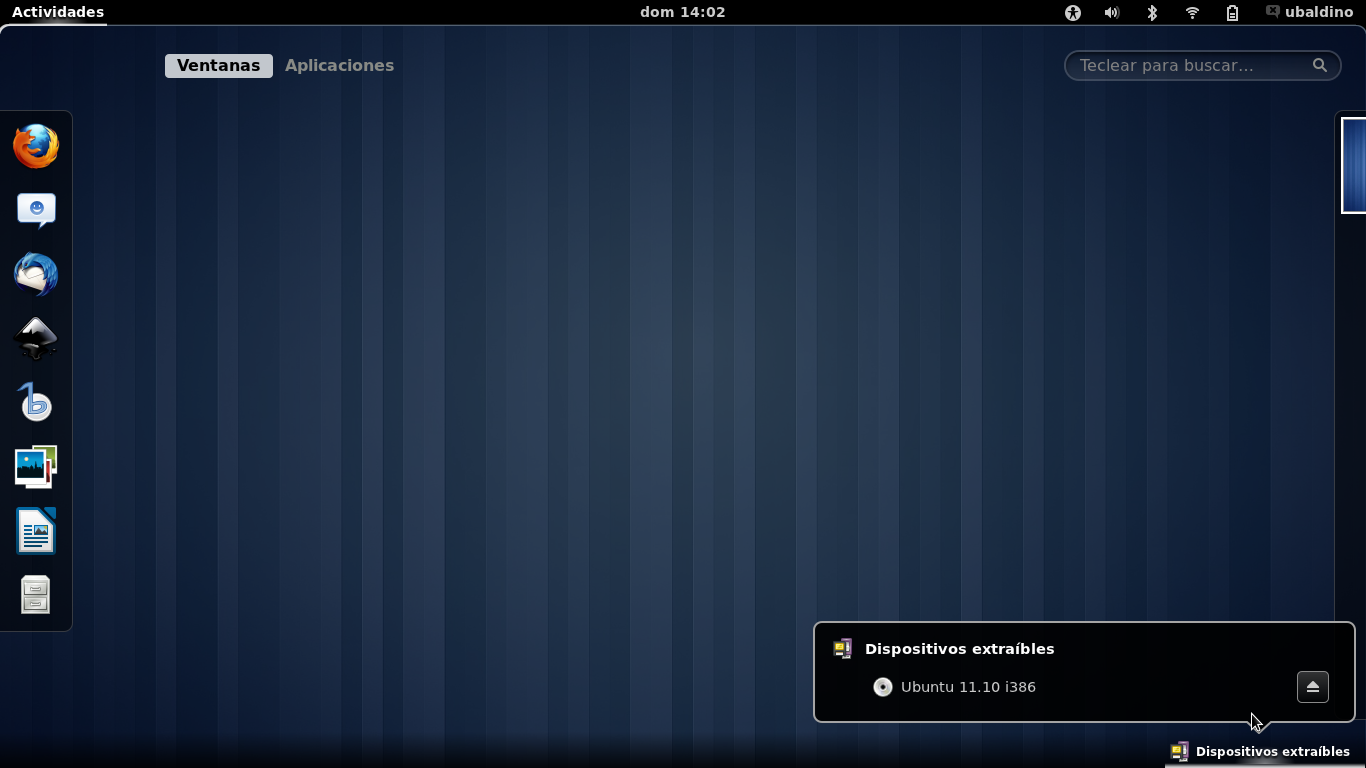
\includegraphics[scale=0.3]{img/Pantallazo7.png} 
\end{center}
\end{itemize}
\section{Ventanas y áreas de trabajo}
Como otros escritorios, GNOME usa ventanas para mostrar las aplicaciones en ejecución. Usando la vista y el tablero, puede lanzar aplicaciones nuevas y controlar qué ventana está activa.\\

Además de en las ventanas, también puede agrupar sus aplicaciones en áreas de trabajo. Visite los temas de ayuda de ventana y área de trabajo que se muestran a continuación para aprender mejor cómo usar estas características.

\subsection{Trabajar con ventanas}
\begin{center}
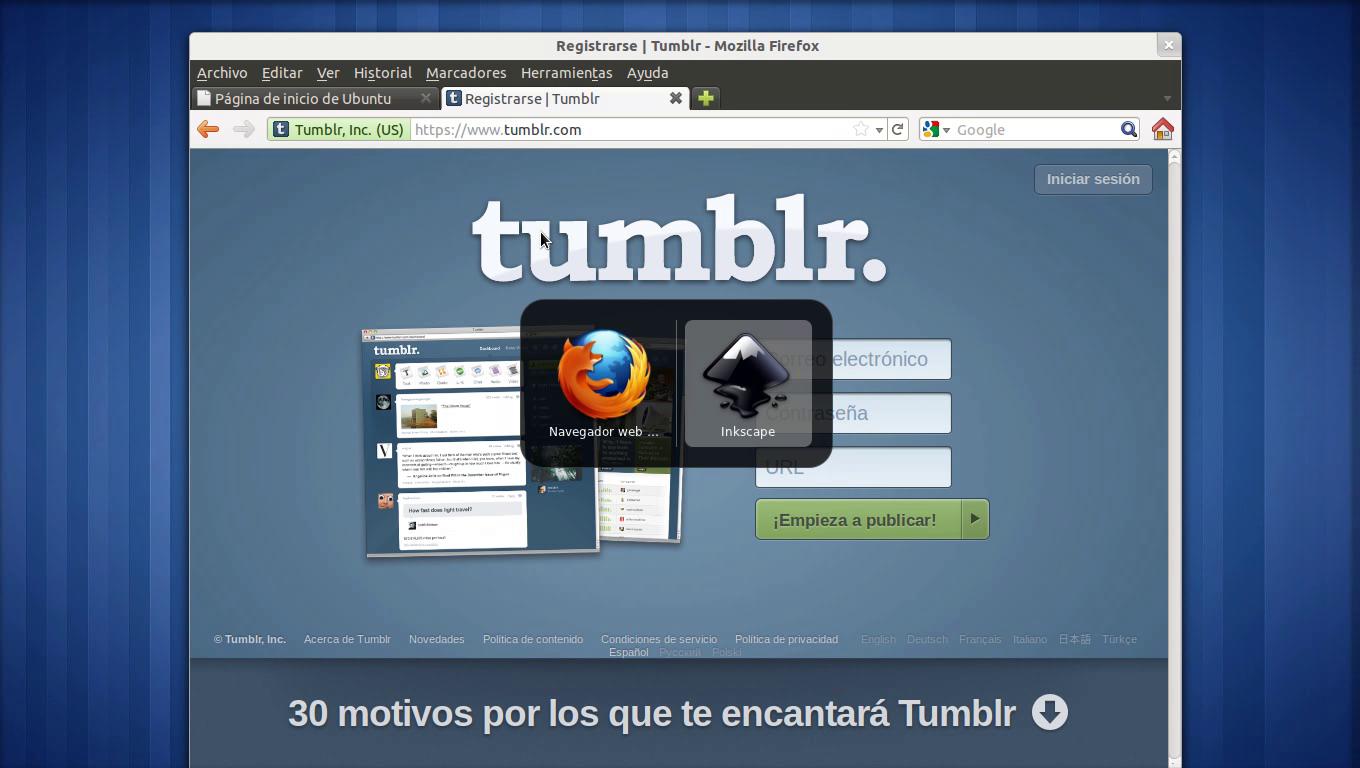
\includegraphics[scale=0.3]{img/ventanas.png} 
\end{center}
\subsubsection{Cambiar entre ventanas}
Incluir todas las aplicaciones en el selector de ventanas hace que el cambio entre tareas sea un proceso sencillo y proporciona una imagen completa de las aplicaciones que están en ejecución.\\

{\bf Desde un área de trabajo:}
\begin{itemize}
\item Pulse Alt+Tab para mostrar el selector de ventanas.
\item Suelte la tecla Alt para seleccionar la siguiente ventana (resaltada) en el selector.
\item Otra forma, aún manteniendo pulsada la tecla Alt, pulse Tab para cambiar entre la lista de ventanas abiertas, o pulse Mayús+Tab para cambiar hacia atrás.
\end{itemize}
Las ventanas en el selector de ventanas se agrupan por aplicaciones. Las vistas previas de las aplicaciones con múltiples ventanas se despliegan cuando las pulsa. Pulse Alt y pulse la tecla Tab para recorrer la lista.\\
En el selector de ventanas, las aplicaciones de diferentes áreas de trabajo se dividen con separadores verticales.

\begin{itemize}
\item También puede moverse entre los iconos de aplicaciones en el selector de ventanas con las teclas $→$ o $←$, o seleccionar una pulsándola con el ratón.\\
Las vistas previas de las aplicaciones con una sola ventana se pueden mostrar con la tecla $↓$.
\end{itemize}
{\bf Desde la vista de Actividades:}
\begin{itemize}
\item Pulse en una ventana para cambiar a ella y salir de la vista previa. Si tiene varias áreas de trabajo abiertas, puede pulsar en cada una de ellas para ver las ventanas abiertas en cada área de trabajo.
\end{itemize}
\subsubsection{Encontrar una ventana perdida}
Una ventana en un área de trabajo diferente, u oculta detrás de otra ventana es sencilla de encontrar usando la vista de actividades:
\begin{itemize}
\item Abra la vista de actividades y asegúrese de que la vista de Ventanas está seleccionada. Si la ventana que está buscando está en el área de trabajo, se mostrará aquí como una miniatura. Para mostrarla de nuevo, simplemente pulse la miniatura, o
\item Pulse en diferentes áreas de trabajo en el selector de áreas de trabajo en la derecha de la pantalla para tratar de encontrar la ventana, o
\item Pulse con el botón derecho en la aplicación en el tablero y se listarán las ventanas abiertas. Pulse en la ventana de la lista a la que quiere cambiar.
\end{itemize}

{\bf Usando el selector de ventanas:}
\begin{itemize}
\item Pulse Alt+Tab para mostrar el selector de ventanas. Mantenga pulsada la tecla Alt y pulse Tab para cambiar entre la lista de ventanas abiertas, o pulse Mayús+Tab para cambiar hacia atrás.
\item Si una aplicación tiene múltiples ventanas abiertas, pulse Alt y la tecla Tab para pasar por ellas.
\end{itemize}
\subsubsection{Maximizar y des-maximizar (restaurar) una ventana}
Para maximizar o restaurar una ventana:
\begin{itemize}
\item Doble pulsación en la barra de títulos de la ventana.
\end{itemize}
Alternativamente, para maximizar:
\begin{itemize}
\item Pulse en la barra de título de una aplicación y arrástrela a la parte superior de la pantalla. Cuando el puntero del ratón toque la parte superior de la pantalla, toda la pantalla se iluminará. Suelte el botón del ratón para maximizar la pantalla.
\end{itemize}
Para restaurar la ventana a su tamaño original:
\begin{itemize}
\item Pulse en la barra de título de la aplicación y arrástrela hacia abajo desde la barra superior. Una vez separada de la barra superior volverá a un estado des-maximizado.
\end{itemize}
Pulse Alt y arrastre con el ratón en cualquier lugar de la ventana. Esto el permitirá mover la ventana. Algunas personas pueden encontrar esto más sencillo que pulsar en la barra de título de una aplicación.\\
También puede usar su teclado para maximizar una ventana. Pulse Alt+Espacio para mostrar el menú de la ventana, y pulse x.
\subsubsection{Operaciones de ventanas}
Las ventanas pueden redimensionarse u ocultarse para ajustarse a un flujo de trabajo
\begin{itemize}
\item {\bf Minimizar, restaurar y cerrar}\\
Para minimizar una ventana u ocultar una ventana:
\begin{itemize}
\item Pulse Alt+Space para mostrar el menú de la ventana. Entonces pulse n. La ventana desaparece en la esquina superior izquierda.
\end{itemize}
Para restaurar la ventana:
\begin{itemize}
\item Pulse en ella o en la vista de actividades o recupérela desde el selector de ventanas pulsando Alt+Tab.
\end{itemize}
Para cerrar la ventana:
\begin{itemize}
\item Pulse en la x en la esquina superior derecha de la ventana, o
\item Pulse Alt+F4, o
\item Pulse Alt+Espacio para mostrar el menú de la ventana. Entonces pulse la tecla c.
\end{itemize}
\item {\bf Redimensionar}\\
Si una ventana está maximizada no se puede redimensionar.\\

Para redimensionar su ventana horizontal y/o verticalmente:
\begin{itemize}
\item Mueva el puntero del ratón a cualquier esquina de la ventana hasta que se convierta en un \underline{puntero de esquina}. Pulse, mantenga y arrastre para cambiar el tamaño de la ventana en cualquier dirección.
\end{itemize}
Para redimensionar sólo horizontalmente:
\begin{itemize}
\item Mueva el puntero del ratón a cualquier lado de la ventana hasta que se convierta en un \underline{puntero lateral}. Pulse $+$ mantenga $+$ arrastre para cambiar el tamaño de la ventana en la dirección horizontal.
\end{itemize}
Para redimensionar sólo verticalmente:
\begin{itemize}
\item Mueva el puntero del ratón a la parte superior o inferior de la ventana hasta que se convierta en un \underline{puntero superior} o en un \underline{puntero inferior}, respectivamente. Pulse, mantenga y arrastre para cambiar el tamaño de la ventana en la dirección vertical.
\end{itemize}
\item {\bf Organizar ventanas en su área de trabajo}\\
Puede situar dos ventanas juntas. Arrastre una ventana por su barra de título hacia la izquierda hasta que el cursor toque el lado izquierdo de la pantalla. La mitad izquierda de la pantalla se iluminará. Suelte el ratón y la ventana se redimensionara para ocupar exactamente la mitad de su pantalla. Haga lo mismo para la otra ventana, arrastrándola a la derecha y soltando.
\end{itemize}
\subsubsection{Ventanas en mosaico}
Su forma de trabajo puede necesitar dos ventanas lado a lado para comprar resultados. Para llenar la pantalla con dos ventanas orientadas verticalmente:
\begin{itemize}
\item Pulse en la barra de título de una aplicación y arrástrela a la parte superior de la pantalla. Cuando el puntero del ratón toque la parte superior de la pantalla, toda la pantalla se iluminará. Suelte el botón del ratón para maximizar la pantalla.
\item Arrastre otra ventana a la parte derecha: cuando la mitad derecha de la pantalla esté resaltada, suélte la ventana. Cada una de las dos ventanas llena la mitad de la pantalla.
\end{itemize}
Pulsar Alt + y pulsar en cualquier parte de una ventana le ayudará a mover la ventana. Algunas personas pueden encontrar esto más sencillo que pulsar en la barra de título de una aplicación.
\subsection{Trabajar con áreas de trabajo}
\begin{center}
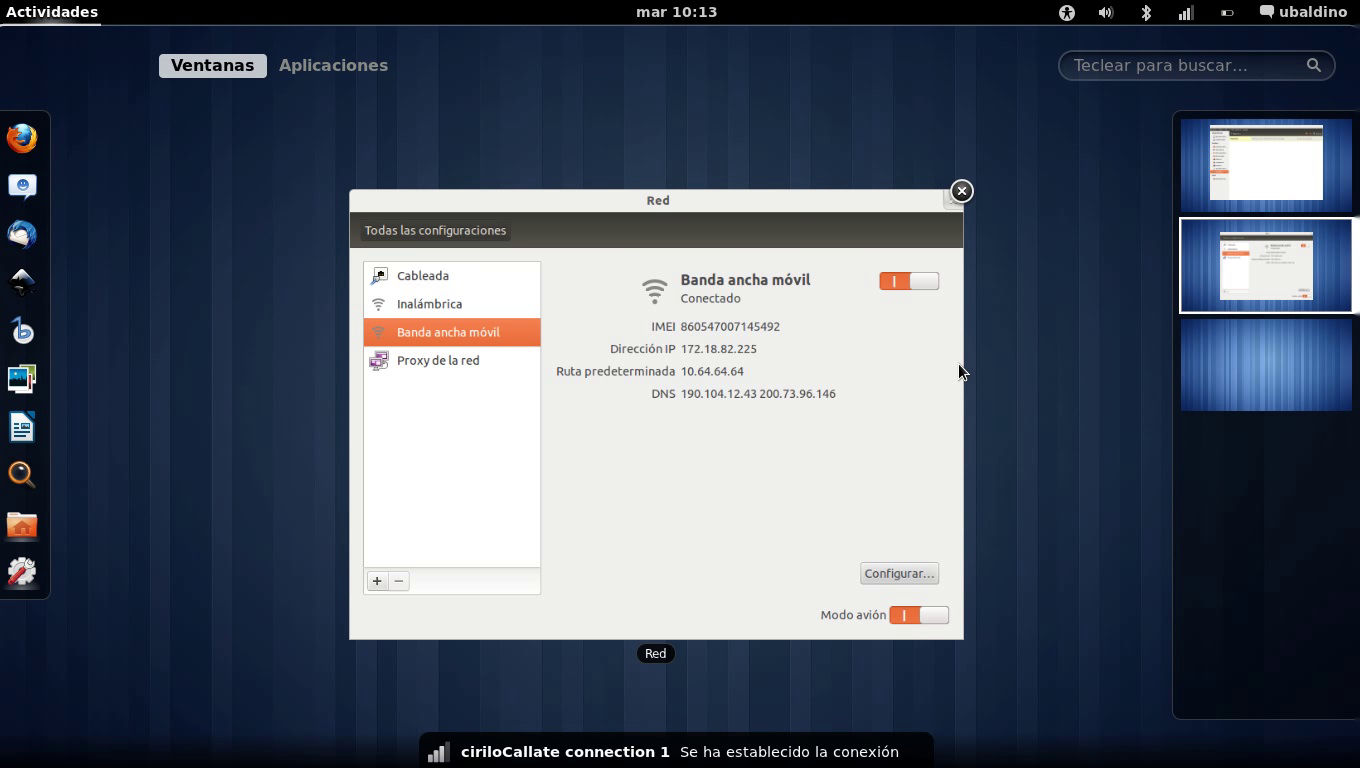
\includegraphics[scale=0.3]{img/areasTr.png} 
\end{center}
\subsubsection{¿Que es un área de trabajo y cómo me ayudará?}
Las áreas de trabajo se refieren a la agrupación de ventanas en su escritorio. Puede crear muchas áreas de trabajo, las cuales actúan como escritorios virtuales. Las áreas de trabajo están destinadas a reducir el desorden y hacer que el escritorio sea sencillo de examinar.\\

Podría utilizar las áreas de trabajo para organizar su trabajo. Por ejemplo, podría tener todas sus ventanas de comunicación, tales como el correo electrónico y su programa de chat en un área de trabajo y el trabajo que está haciendo en un área de trabajo diferente. Su gestor de música podría estar en una tercera área de trabajo.\\

{\bf Usando áreas de trabajo:}
\begin{itemize}
\item En la vista de Actividades, mueva su cursor a la parte más a la derecha de la pantalla. Aparecerá un panel vertical con las áreas de trabajo en uso y con área de trabajo adicional vacía. Esto es el selector de áreas de trabajo.
\item Para añadir un área de trabajo, mueva una ventana de un área de trabajo existente hasta el área de trabajo vacía en el selector de áreas de trabajo. Esta área de trabajo contiene ahora la ventana que se dejó en ella, y debe aparecer un área de trabajo nueva vacía en la parte inferior.
\item Para quitar un área de trabajo, simplemente cierre todas las ventanas que tenga, o muévalas a otras áreas de trabajo.
\end{itemize}
Siempre hay al menos un área de trabajo.
\subsubsection{Cambie entre las áreas de trabajo}
\begin{itemize}
\item {\bf Usando el ratón:}\\
En la vista Actividades, pulse en un área de trabajo en el selector de áreas de trabajo en el lado derecho de la pantalla para ver las ventanas abiertas en ese área de trabajo. Pulse en cualquier miniatura de ventana para activar el área de trabajo.\\

\item {\bf Usando el teclado:}
\begin{itemize}
\item Pulse Ctrl+Alt+$↑$ para moverse a un área de trabajo que esté encima de la actual en el selector de áreas de trabajo.
\item Pulse Ctrl+Alt+$↓$ para mover a un área de trabajo que está debajo del área de trabajo actual en el selector de áreas de trabajo.
\end{itemize}
\end{itemize}
\subsubsection{Mover una ventana a un área de trabajo diferente}
\begin{itemize}
\item {\bf Usando el ratón:}
\begin{enumerate}
\item Abra la vista de Actividades y asegúrese de que está en la vista de Ventanas.
\item Pulse y arrastre la ventana a la derecha de la pantalla.
\item El selector de áreas de trabajo aparecerá.
\item Arrastre la ventana a un área de trabajo vacía. Este área de trabajo ahora contiene la ventana que se arrastró en ella y se creará una nueva área de trabajo vacía al final del selector de áreas de trabajo.
\end{enumerate}
\item {\bf Usando el teclado:}
\begin{enumerate}
\item Pulse sobre la ventana para hacerla activa.
\item Pulse Ctrl+Alt+Mayús+$↑$ para mover la ventana al área de trabajo encima del actual en el selector de áreas de trabajo.
\item Pulse Ctrl+Alt+Mayús+$↓$ para mover la ventana al área de trabajo debajo del actual en el selector de áreas de trabajo.
\end{enumerate}
\end{itemize}